\documentclass[mathserif]{beamer}

\usepackage[utf8]{inputenc}
\usepackage{graphicx}
\usepackage{mathtools}
\usepackage{amsthm}
\usepackage{algorithmic}


\usetheme{default}
\usecolortheme{beaver}


\title{Time-independent Schrödinger Equation in 2D}
\subtitle{Particle in a Box}

\author{Julien Brenneck}

\beamertemplatenavigationsymbolsempty

\date{Math/ECE 697NA, Spring 2017}


\subject{Numerical Linear Algebra}
% This is only inserted into the PDF information catalog. Can be left
% out. 


\begin{document}

\begin{frame}
  \titlepage
\end{frame}



\section{Intro}

\subsection{1D Problem}

\begin{frame}{1D Problem}{Infinite potential well}
  Particle trapped in a 1D well, with walls of infinite potential to either side. Size of problem $L=1 \times 10^{-9}$ m \\
    \begin{figure}
    \centering
    \def\svgwidth{15em}
    \input{1d.pdf_tex}
    \end{figure}
\end{frame}

\begin{frame}{1D Problem}{Infinite potential well}
  Particle has probability distribution for each energy level. \\
  For a $1 \times N$ grid we get $N^2$ entries in our matrix. \\
  \center \includegraphics[scale=0.4]{1dp.pdf}
\end{frame}

\subsection{2D Problem}

\begin{frame}{2D Problem}{Particle in a box}

The problem is the same in 2D, we get probability distributions for a particle in the well. For a $N \times N$ grid our matrix is size $N^4$. \\
\center 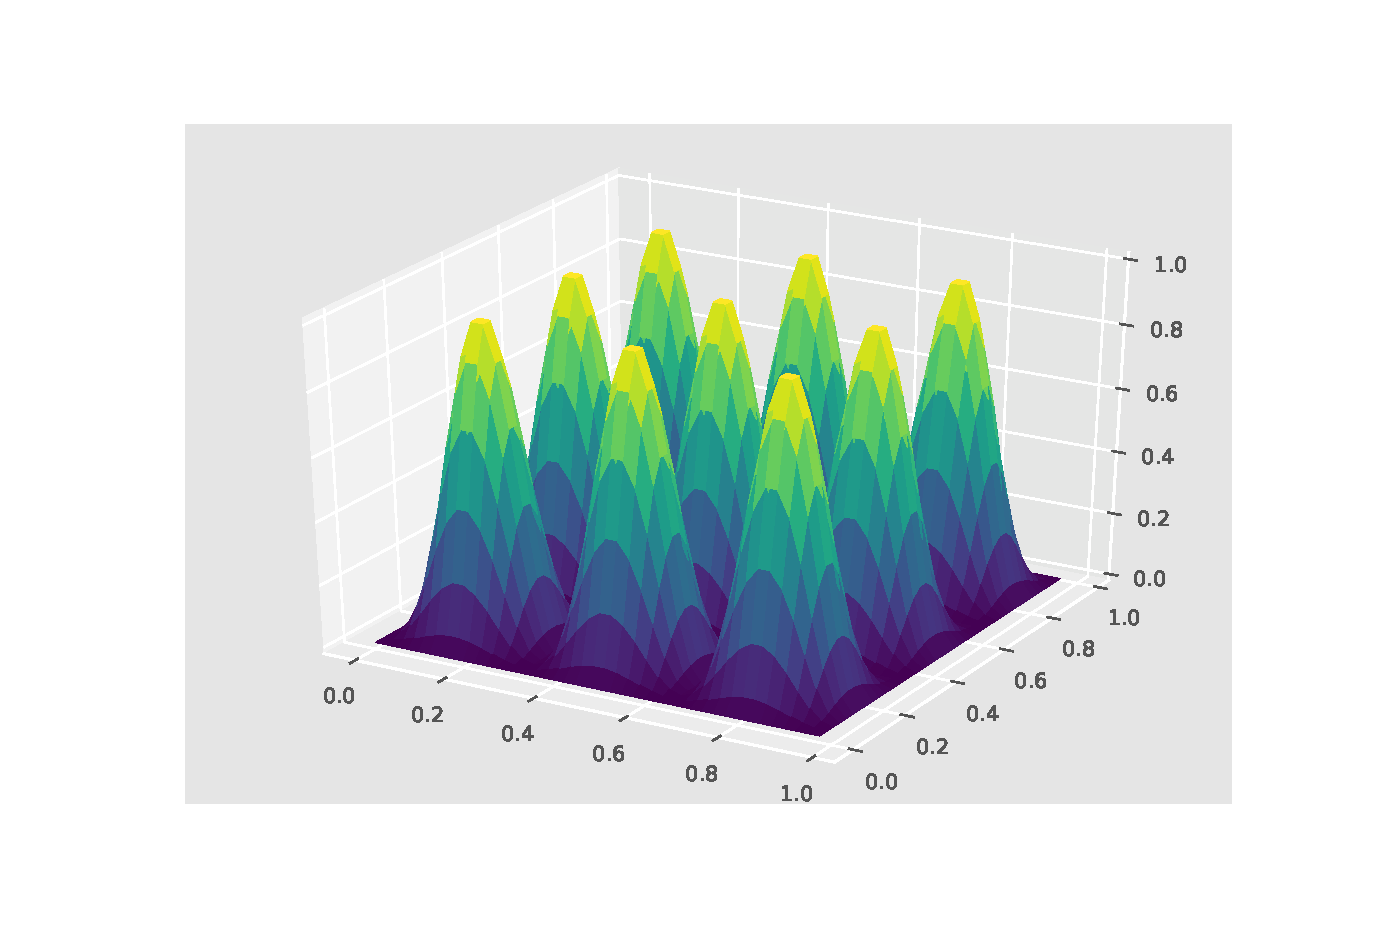
\includegraphics[scale=0.4]{2dp.eps}
  
\end{frame}

\begin{frame}{Schrödinger Equation}
The wave function is given by the Schrödinger equation, which can be viewed as an eigenvalue problem. \\

$$ - \frac{\hbar}{2 m_e} \Delta \Psi + U \Psi = E \Psi$$
$$ \left[- \frac{\hbar}{2 m_e} \Delta + U \right] \Psi = E \Psi$$
$$ A \Psi = E \Psi$$
  
\end{frame}

\begin{frame}{Schrödinger Equation}{1D Analytical Solution}
For a constant zero potential in the well $U = 0$, the equation is separable and we can find an analytical solution.

$$E_i = \frac{(i \pi \hbar)^2}{2 m_e L^2}$$
$$ \psi_i (x) = \sqrt{\frac{2}{L}} \sin \left( \frac{i \pi x }{L} \right)$$
  
\end{frame}

\begin{frame}{Schrödinger Equation}{2D Analytical Solution}
For a constant zero potential in the well $U = 0$, the equation is separable and we can find an analytical solution.

$$E_{i,j} = \frac{(i \pi \hbar)^2}{2 m_e L^2}+\frac{(j \pi \hbar)^2}{2 m_e L^2}$$
$$ \psi_{i,j} (x) = \sqrt{\frac{4}{L^2}} \sin \left( \frac{i \pi x }{L} \right) \sin \left( \frac{j \pi x }{L} \right)$$
  
\end{frame}

\begin{frame}{Schrödinger Equation}{2D Eigenvalues}
First 25 Eigenvalues. Since the pairs are symmetric, values appear more than once.

\center \includegraphics[scale=0.4]{Ea25.eps}

  
\end{frame}

\begin{frame}{Schrödinger Equation}{2D Eigenvectors}
First 4 eigenvectors. We take $| \psi_{i,j}(x) |^2$ to get the probability distribution.

\center 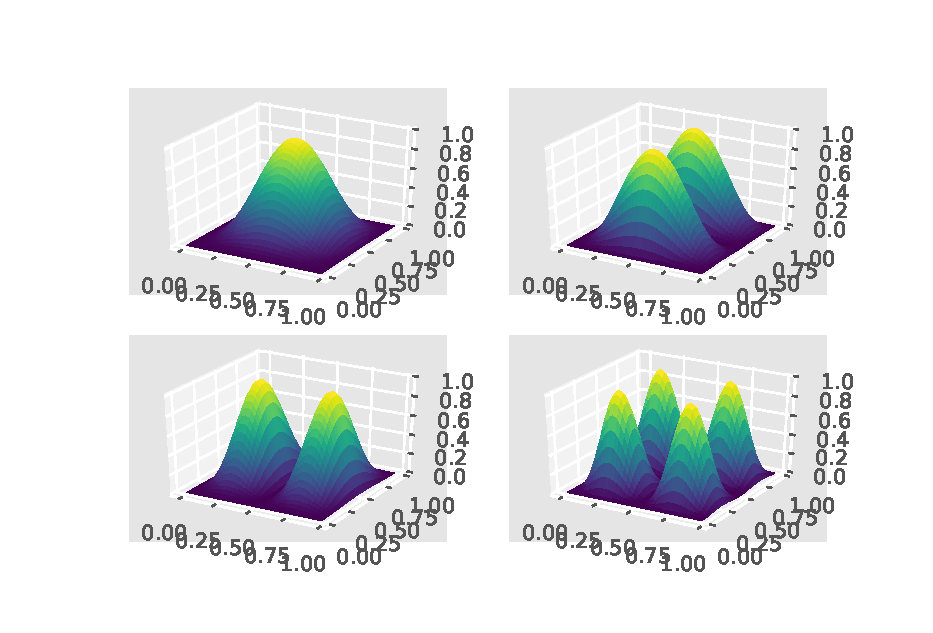
\includegraphics[scale=0.6]{psi1234.eps}

  
\end{frame}

\section{Solve with Finite Difference}

\subsection{Finite Difference}

\begin{frame}{Finite Difference Method}
We can solve this by using a finite difference method to approximate the Laplacian. 

$$A = 
\frac{1}{h^2}
\begin{pmatrix}
4 + U & -1 & 0 & \hdots & -1 & 0 & \hdots \\
-1 & 4 + U & -1 & 0 & \hdots & -1 & 0 & \hdots \\
0 & -1 & 4 + U & -1 & 0 & \hdots  & \ddots \\
\vdots & 0 & -1 & 4 + U & -1 & 0 & \hdots  \\
-1 & 0 & \hdots & -1 & 4 + U & -1 & 0 & \hdots  \\
0 & -1 & \hdots &  &  & \ddots &  &  \\
\vdots & 0 & \ddots &  &  & & \ddots &  \\
\end{pmatrix}
$$
  
\end{frame}

\begin{frame}{Finite Difference Method}
We can solve this by using a finite difference method to approximate the Laplacian. 

$$A = 
\frac{1}{h^2}
\begin{pmatrix}
B & -I & 0 & \hdots \\
-I & B & \ddots  \\
0 & \ddots & \ddots & -I \\
\vdots &  & -I & B \\
\end{pmatrix}
$$

\end{frame}

\begin{frame}{Finite Difference Method}
Since the problem is the same in both dimensions, the 2D Laplacian can be computed as a tensor product of 1D Laplacians.

$$ L_2 = L_1 \oplus L_1 = L_1 \otimes I + I \otimes L_1 $$

\end{frame}


\begin{frame}{Finite Difference Method}
We can then solve $A \psi = E \psi$ using FEAST, ARPACK, Lanczos algorithm, or other sparse eigenvalue methods. The error increases for larger eigenvalues. 

\center 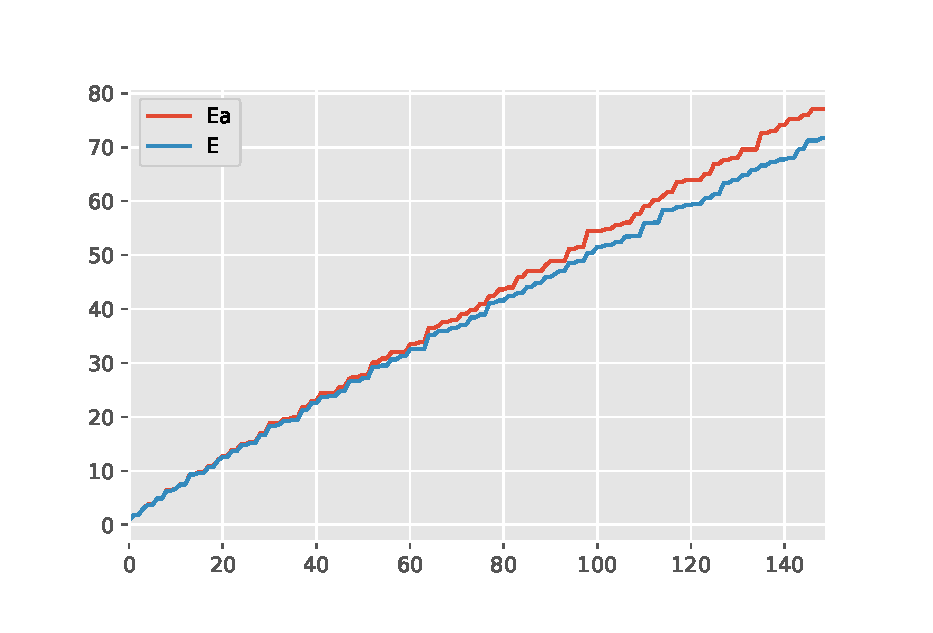
\includegraphics[scale=0.5]{EEa.eps}

\end{frame}


\subsection{Lanczos}

\begin{frame}{Lanczos Algorithm}

\begin{algorithmic}
\STATE $v_1 \gets \texttt{random vector of norm 1}$
\STATE $v_0 \gets 0$
\STATE $\beta_1 \gets 1$
\FOR {$j = 1,2, \cdots, m$} 
    \STATE $w_j' \gets Av_j - \beta_j v_{j-1}$
    \STATE $\alpha_j \gets {w_j'}^T \cdot w_j$
    \STATE $w_j \gets w_j' - \alpha_j v_{j}$
    \STATE $\beta_{j+1} \gets ||w_j'||$
    \STATE $v_{j+1} \gets w_j'/\beta_{j+1}$
\ENDFOR
\end{algorithmic}

\end{frame}


\begin{frame}{Summary}

\center 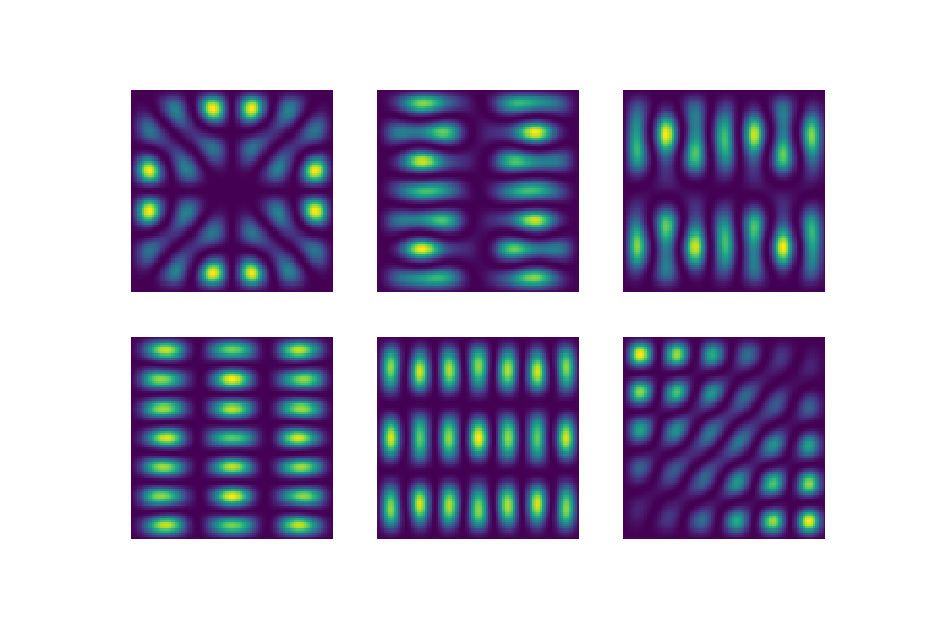
\includegraphics[scale=0.7]{what.eps}

\end{frame}

\begin{frame}{Summary}

\center 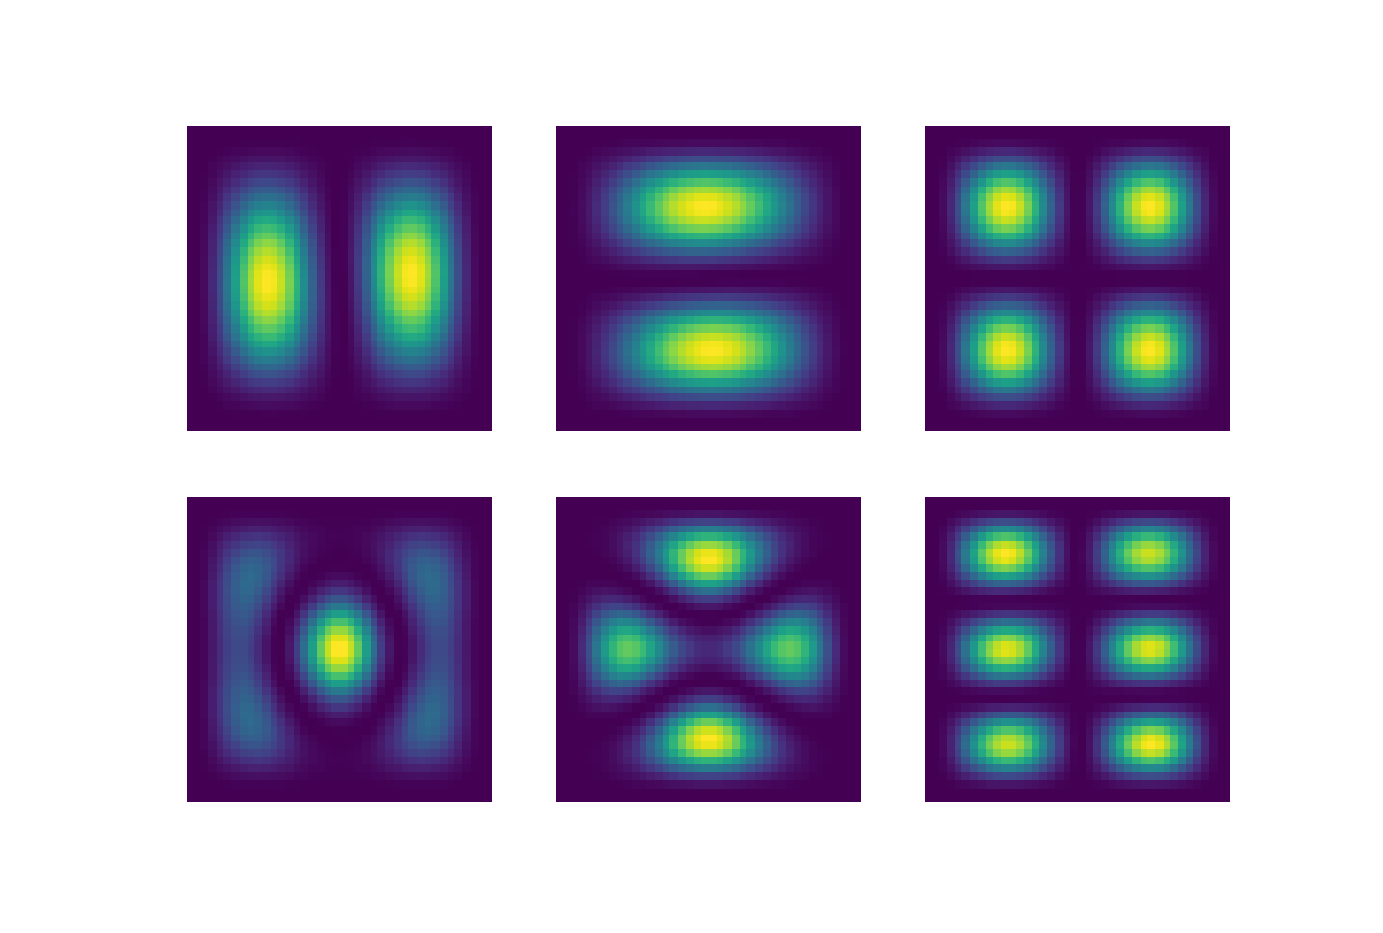
\includegraphics[scale=0.45]{what1.eps}

\end{frame}

\begin{frame}{Summary}

\center 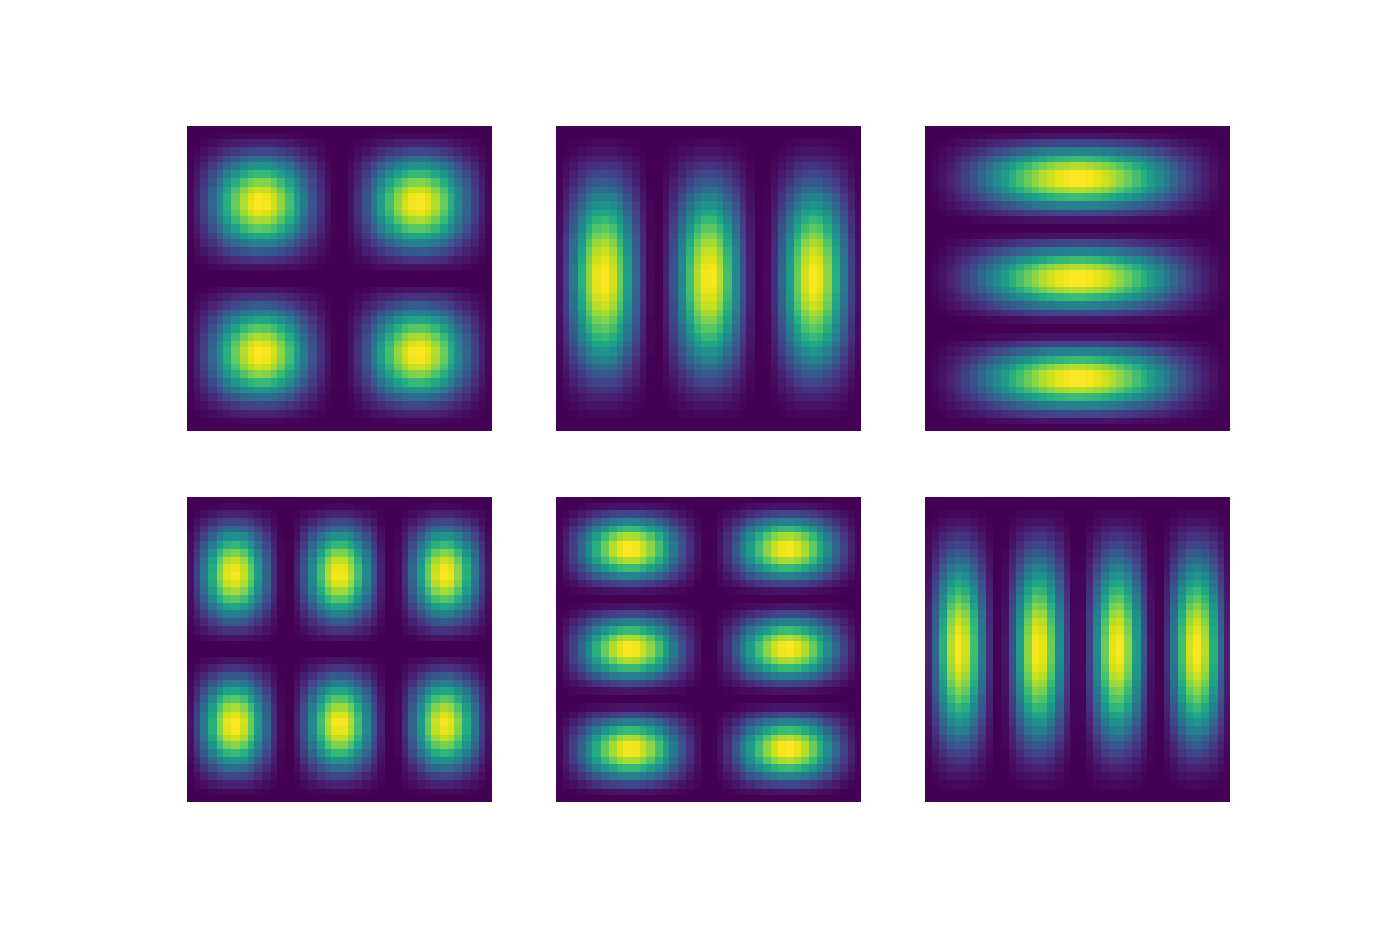
\includegraphics[scale=0.45]{correct3.eps}

\end{frame}

\begin{frame}{Summary}

\center 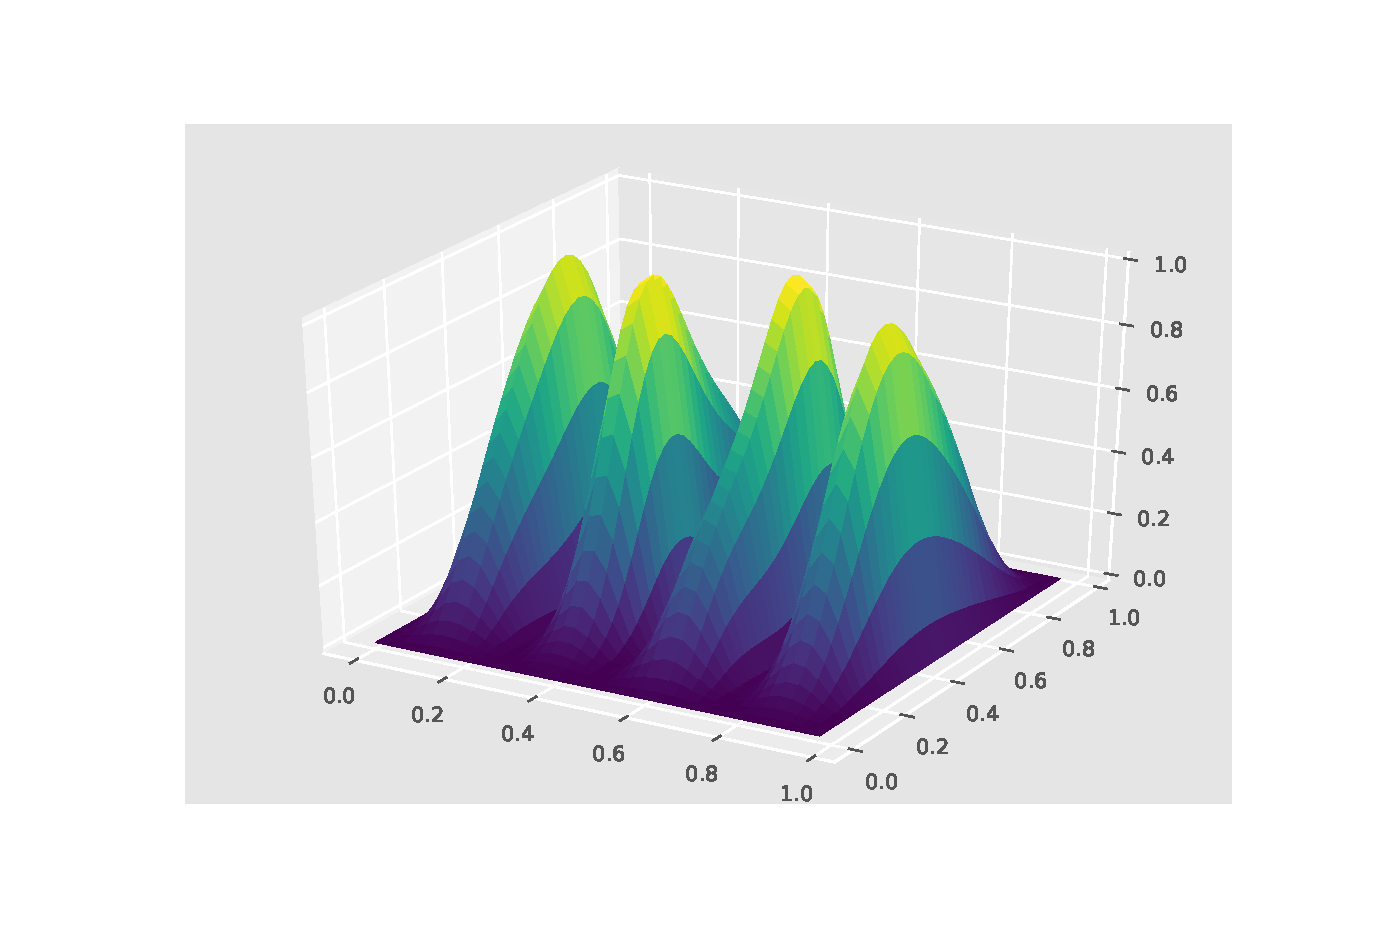
\includegraphics[scale=0.45]{psi8.eps}

\end{frame}

\begin{frame}{Summary}

\center 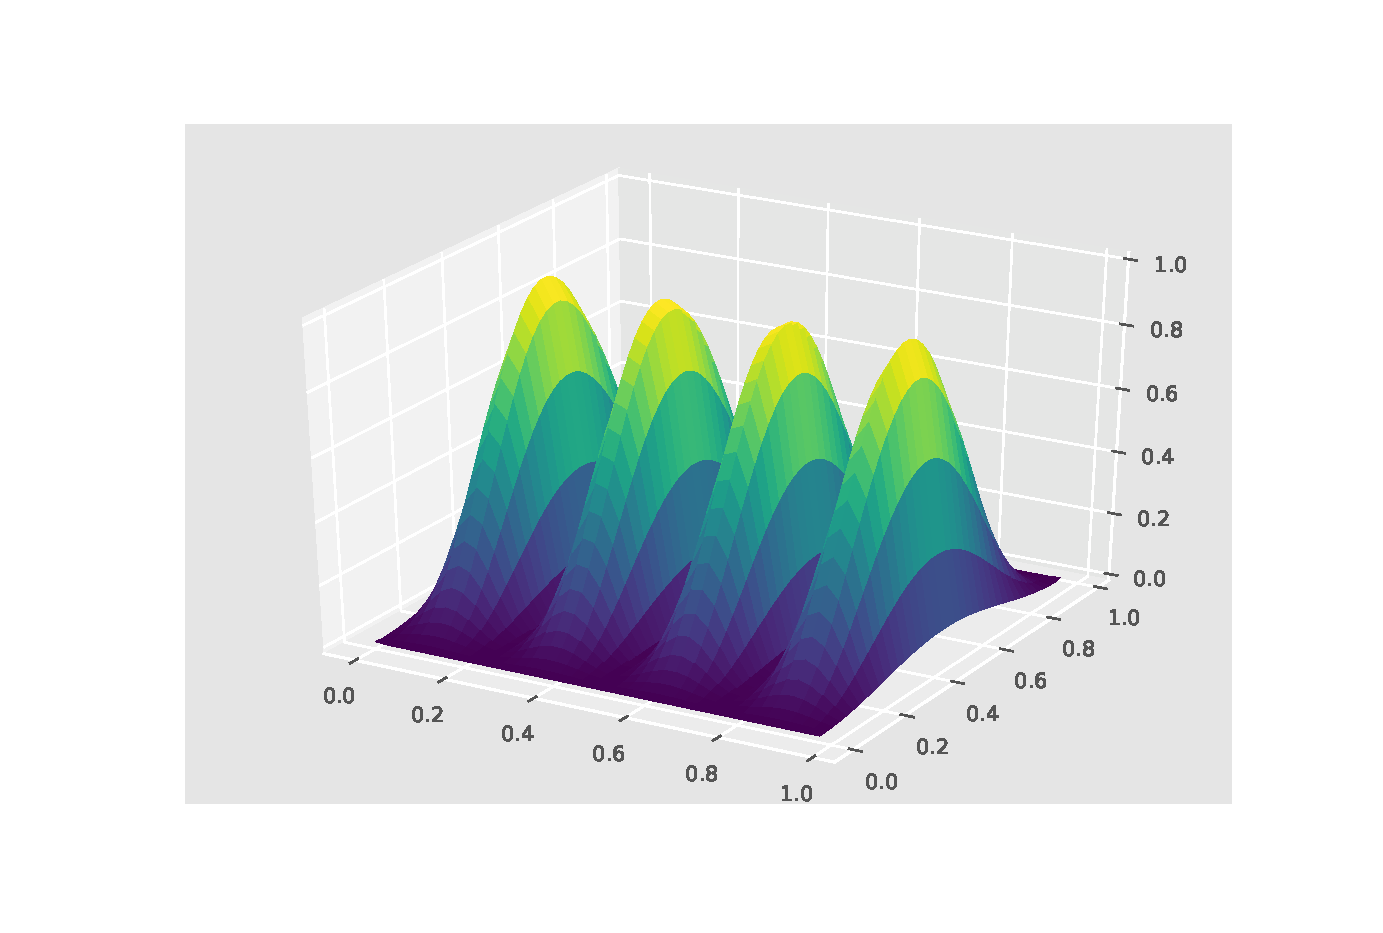
\includegraphics[scale=0.45]{psi10.eps}

\end{frame}



\end{document}


